\section{Problema de Valor de Contorno}

A solução de problemas envolvendo um modelo matemático descrito por uma equação ou sistema de equações diferenciais, pode ser obtida  a partir da especificação das condições iniciais ou das condições de contorno do domínio. Tais condições adicionais formalizam respectivamente, os problemas de valor inicial e de valor de contorno relacionados ao modelo em questão.

Para se definir um problema de valor inicial (PVI), dado um modelo de ordem N, é preciso estabelecer em um determinado ponto, os valores da variável dependente e de suas derivadas até a ordem N-1. Se alguma condição for dada em algum ponto diferente do primeiro, tem-se definido o problema de valor de contorno (PVC). Enquanto os PVI geralmente envolvem o tempo como variável independente, os PVC normalmente são definidos em função do espaço e representam a resposta em estado estacionário de um problema variante no tempo.
\citep[p. 447]{boyce_diprima}

Dado o domínio $ \Omega $ tal que

\begin{equation}
  \Omega \subset \Re^{n}
\end{equation}

Os valores na fronteira $ \partial \Omega $ do domínio são definidos por uma função $ u(x, y) $ tal que

\begin{equation}
  u(x, y) = f(x, y),  \forall (x, y) \in \partial \Omega
\end{equation}

Assim, conhecendo-se os valores na borda, é possível inferir o conjunto de funções em $ \Omega $ que seja solução do modelo. 

De forma a exemplificar, considere o caso simples, em que o domínio $ \Omega $ seja um intervalo aberto em $ \Re $ e os pontos da fronteira sejam os extremos deste intervalo: 

\begin{equation}
  [a, b] \subset \Re
\end{equation}

\begin{equation}
  \Omega = [a, b]
\end{equation}

\begin{equation}
  \partial [a, b] = \{ a, b \}
\end{equation}

Um problema de valor de contorno definido sobre este domínio é portanto, composto pela equação que modela o comportamento do processo e pelas condições adicionais de contorno


\begin{equation}
    \label{eq:pvc}
    PVC = 
    \begin{cases}
        y'' = f(x, y, y') \\
        y(a) = \alpha \\
        y(b) = \beta
    \end{cases}
\end{equation}

Conforme mostra a figura ~\ref{fig:pvc}, a solução para o exemplo dado, consiste em encontrar a curva ou o conjunto de curvas que obedeçam às condições de contorno.

\begin{figure}[ht!]
\centering
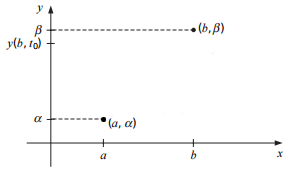
\includegraphics[scale=0.8]{figuras/PVC.png}
\caption{PVC: Encontrar a curva solução entre os pontos $ \alpha $ e $ \beta $}
\label{fig:pvc}
\end{figure}
